%\renewcommand{\thefootnote}{\arabic{footnote}}
\chapter{TINJAUAN PUSTAKA}
\label{BAB2:tinjauan}

\lipsum[3-4]
\begin{equation}
  L(x,W)= \frac{1}{N}\sum\limits_{i=0}^{N} l(x_i,W)   
  \label{func:loss}
\end{equation}

\lipsum[5-6]
\begin{table}[h]
    \centering
    \caption{Rata-rata loss dan accuracy Model A untuk seluruh round}
\begin{tabularx}{0.95\textwidth} { 
  | >{\centering\arraybackslash}X 
  | >{\centering\arraybackslash}X | }
 \hline
  train\_accuracy &	0.46846 \\
 \hline
  train\_loss &	2.71451 \\
 \hline
  val\_accuracy &	0.47391 \\
  \hline
  val\_loss & 2.69424 \\
  \hline
\end{tabularx}
    \label{tab:my_label}
\end{table}

\lipsum[7]
\begin{center}
\begin{figure}[h]
    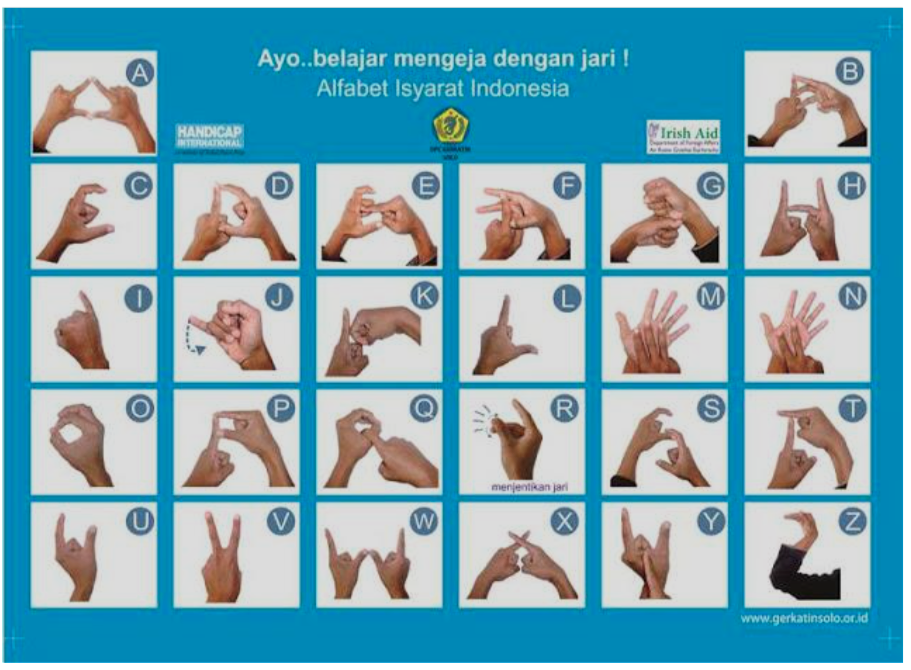
\includegraphics[width=\textwidth]{BAB-2/figures/alfabetbisindo.png}	
	    \caption{Alfabet Bisindo (Almuharram, 2013).}
	    \label{gambar:alfabet bisindo}
\end{figure}
\end{center}
Gambar \ref{gambar:alfabet bisindo} menyunjukkan sudut pandang umum yang digunakan dalam berkomunikasi menggunakan bahasa isyarat, yaitu tampak depan \citep{xiong2004_dscForSensorNetworks}. Sehingga, data gambar yang digunakan di penelitian ini juga memuat gestur Bisindo dari tampak depan, dengan persamaan~(\ref{func:loss}), dengan hasil penelitian di Bab~\ref{BAB4:hasil}.